\item {\bf Boxcar Averager} A sliding window averager has a window length of
three samples.  

\begin{enumerate}
\item Using Matlab, plot, on the same axes, the input and output of
this averager given the input samples listed below. Assume that the input at
times \textit{before} and \textit{after} these samples is equal to zero. \\

\centerline{0~~ 0.2~~ 0~~ -0.1~~ 0.3~~ 0.8~~ 1.2~~ 0.9~~ 1.1~~ 1.2~~ 0.8~~ 1.1~~ 1.2~~ 0.8~~ 1.1~~ 0~~ -0.2~~ -0.1~~ 0~~ -0.2~~}

\item If the actual signal trying to be represented by these samples is: \\

\centerline{0.0~~ 0.0~~ 0.0~~ 0.0~~ 0.0~~ 0.0~~ 1.0~~ 1.0~~ 1.0~~ 1.0~~ 1.0~~ 1.0~~ 1.0~~ 0.0~~ 0.0~~ 0.0~~ 0.0~~ 0.0~~ 0.0~~ 0.0~~}

then comment on the pros / cons of the sliding averager relative to recovering
the actual signal.
\end{enumerate}


Qualitatively you observed a reduction in noise, but the quantitative estimate
of SNR improvement did not achieve the theoretical $\sqrt{3}$ because you
didn't take into account what the ``true'' signal should be (I didn't tell you
what is was); performing mean and standard deviation operations over the entire
signal includes the variability of the actual signal (which in this case was a
\verb+rect+).

Remember that SNR =
$\frac{\textrm{P}_{\textrm{signal}}}{\textrm{P}_{\textrm{noise}}}$.  If we look
at the SNR improvement in the data from Problem Set \#6 in the region of the
\verb+rect+ that has actual signal (non-zero values), then we get the
following:

\begin{center}
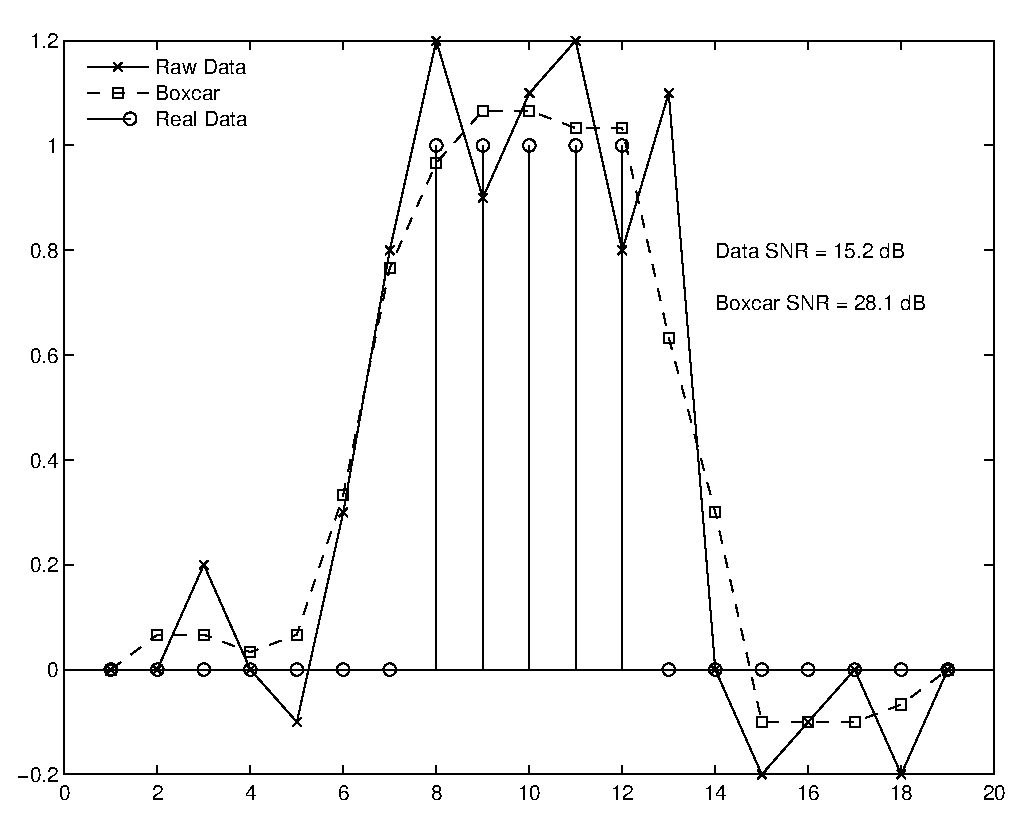
\includegraphics[width=0.5\linewidth]{boxcar_averager/sliding_average.eps}
\end{center}

Looking at the SNRs calculated above, how does the SNR improvement compare with
the ``expected'' $\sqrt{3}$?  Why might this be?

The SNR improvement is $\frac{10^{28.1/20}}{10^{15.2/20}} \simeq 4.4 >
\sqrt{3}$.  This is partially due to the fact that the $\sqrt{N}$ rule-of-thumb
was derived under the assumption of a normal distribution of data points;
having such a small number of points violates that assumption.\\

